\SectionNote{$\bm{\mu}$ is no longer fixed: one network trained once, for all $\bm{\mu}\in\mathcal{M}$}
\section[Parametric case]{Parametric enrichment}

\begin{frame}{Parametric case: principle}
	\rigiddisplayskips{7pt}
	\vspace{-12pt}
	\centering
	\only<1>{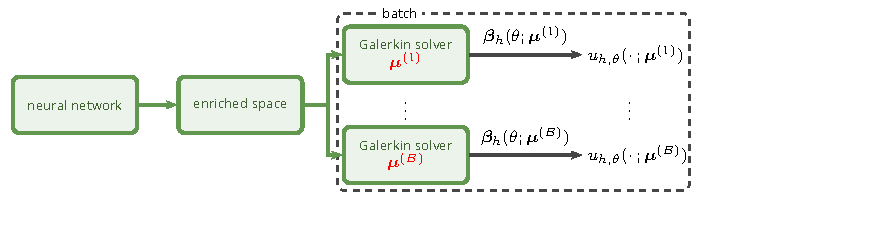
\includegraphics[page=1]{images/contrib2/operator_scheme/operator_scheme.pdf}}%
	\only<2>{\includegraphics[page=2]{images/contrib2/operator_scheme/operator_scheme.pdf}}%
	\only<3>{\includegraphics[page=3]{images/contrib2/operator_scheme/operator_scheme.pdf}}%
	\only<4->{\includegraphics[page=4]{images/contrib2/operator_scheme/operator_scheme.pdf}}

	\vspace{-10pt}
	\raggedright
	\textbf{Parameter sampling:} $\mathcal{D}_\text{train}\subset\mathcal{M}$ chosen once, a random batch of $\bm{\mu}$ drawn at each epoch.

	\vspace{3pt}
	\textbf{Parametric scheme:} \coloredonly<1>{One network, one Galerkin solve per $\bm{\mu}$ of the batch}: $A_h(\theta;\bm{\mu})\,\bm{\beta}_h(\theta;\bm{\mu})=\bm{b}_h(\theta;\bm{\mu}).$

	% \vspace{3pt}
	% \textbf{Discretization:} DG here, each $\phi_i$ supported on a single cell. (SIPG)\quad\refappendix{dg}

	\vspace{3pt}
	\blk{2}{%
	\textbf{Supervised loss:} \coloredonly<2>{Fit reference solutions on the batch}, at $N_x$ points per $\bm{\mu}$:
	\vspace{-3pt}
	\[
		\mathcal{J}_\text{data}(\theta)=\frac{1}{B\,N_x}{\sum_{i=1}^{B}\sum_{j=1}^{N_x}}\Big|u_{h,\theta}\big(\bm{x}^{(j)};\bm{\mu}^{(i)}\big)-u_\text{ref}\big(\bm{x}^{(j)};\bm{\mu}^{(i)}\big)\Big|^2.
	\]
	}

	\vspace{-3pt}
	\blk{3}{%
		\textbf{Gradient:} \coloredonly<3>{one adjoint solve per $\bm{\mu}$} of the batch.
	}
\end{frame}

\begin{frame}{Constructing the enriched space (three ways)}
	\centering
	\only<1>{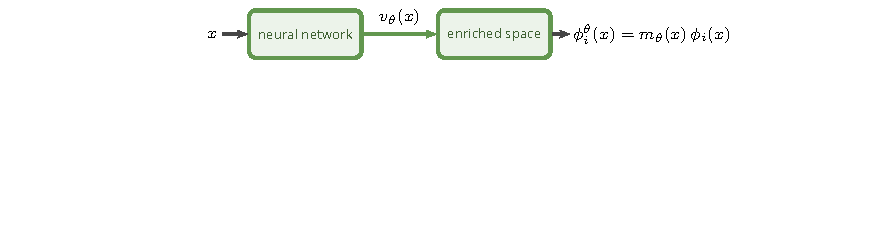
\includegraphics[page=1]{images/contrib2/enriched_bases/enriched_bases.pdf}}%
	\only<2>{\includegraphics[page=2]{images/contrib2/enriched_bases/enriched_bases.pdf}}%
	\only<3->{\includegraphics[page=3]{images/contrib2/enriched_bases/enriched_bases.pdf}}

	\vspace{2pt}
	\raggedright
	\textbf{Shared basis:} \coloredonly<1>{same enriched space} for all $\bm{\mu}$.

	\vspace{2pt}
	\blk{2}{%
		\textbf{$\bm{\mu}$-dependent basis:} \coloredonly<2>{one enriched space per $\bm{\mu}$}.
	}

	\vspace{2pt}
	\blk*{3}{%
		\textbf{Field-dependent basis:} an \coloredonly<3>{encoder} summarizes the transport field in a latent state $\bm{z}$.
	}
\end{frame}

\begin{frame}{1D linear transport}
	\raggedright
	\textbf{Test case:} Same 1D case as the PINN, with $\bm{C}(x,\bm{\mu})=\mu_1+\mu_2x$, $\bm{\mu}\in[0.8,1.2]^2$: the layer \coloredonly<1>{stays at $x=1$}.

	\vspace{2pt}
	\only<1>{\vphantom{$N_\text{cells}$}\par} % réserve la place de Setup : la figure ne bouge pas entre les overlays
	\blk{2}{%
		\textbf{Setup:} DG, $N_\text{cells}=8$, $k=2$, $32$ training $\bm{\mu}$, batch of $16$, $N_x=101$ points per $\bm{\mu}$.%, best of $10$ seeds.
	}

	\vspace{-5pt}
	\parbox[t][4.0cm][c]{\linewidth}{\centering
		\only<1>{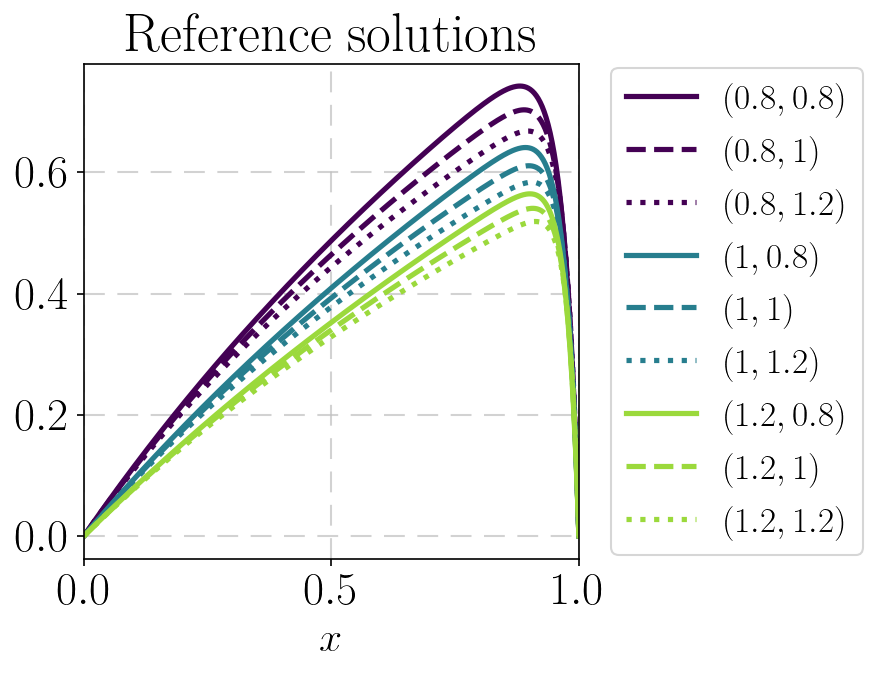
\includegraphics[height=3.7cm]{images/contrib2/operator/lt_reference_solutions.png}}%
		\only<2>{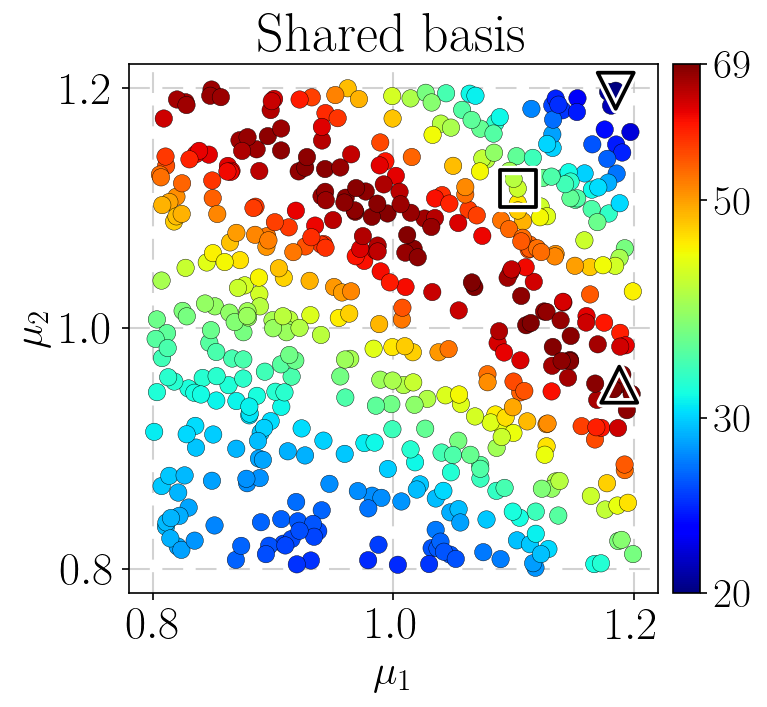
\includegraphics[height=3.35cm]{images/contrib2/operator/lt_gain_map_shared.png}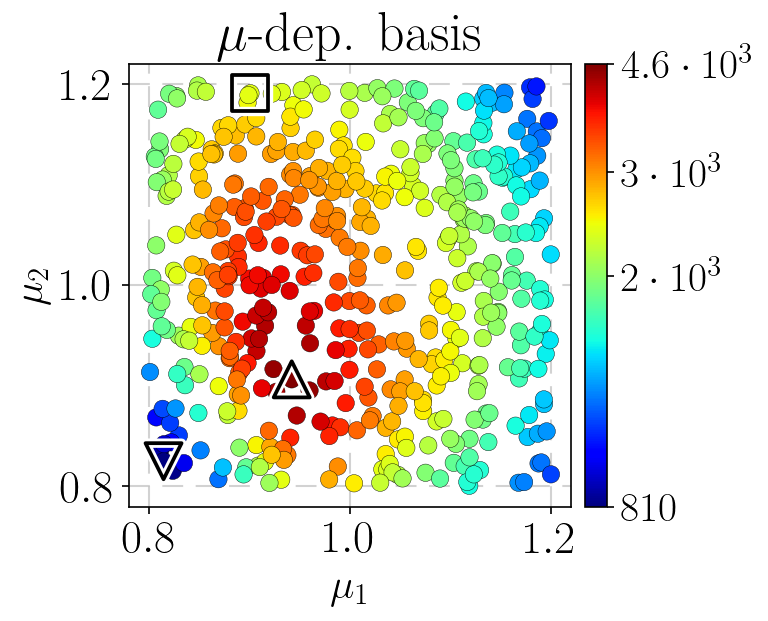
\includegraphics[height=3.35cm]{images/contrib2/operator/lt_gain_map_mu.png}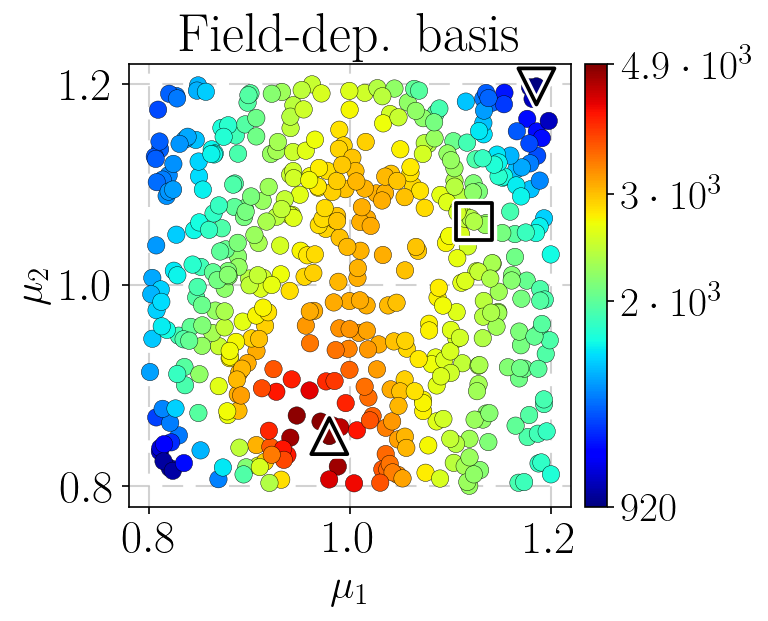
\includegraphics[height=3.35cm]{images/contrib2/operator/lt_gain_map_field.png}\\[2pt]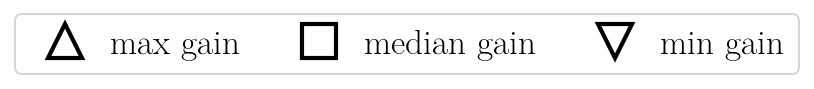
\includegraphics[height=0.5cm]{images/contrib2/operator/lt_gain_map_legend.png}}%
		\only<3->{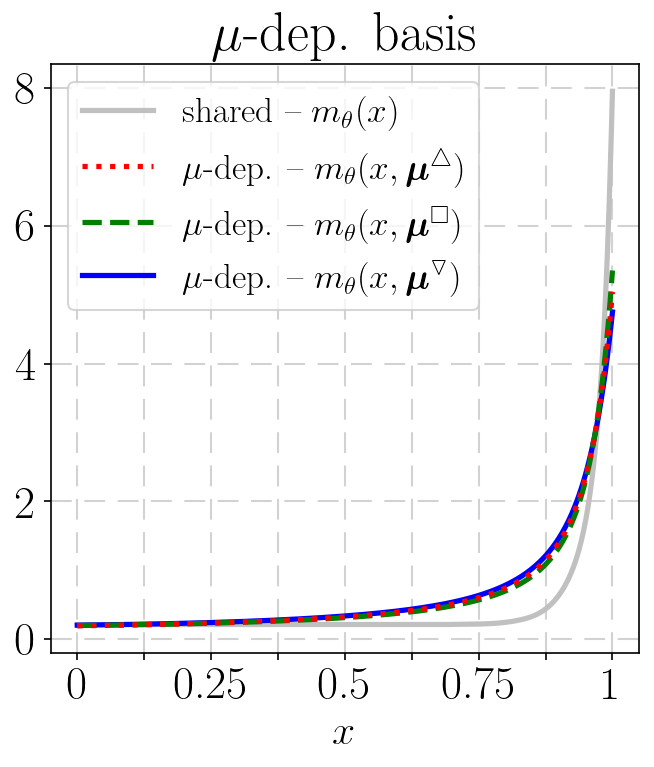
\includegraphics[height=3.9cm]{images/contrib2/operator/lt_multipliers_mu.png}}%
	}

	\vspace{2pt}
	\blk{2}{%
		\textbf{Gain (on $500$ unseen $\bm{\mu}$):} \\
		shared $20$--$69$ $(N_\theta=321)$, \coloredonly<2>{$\bm{\mu}$-dep.\ $811$--$4.6\cdot10^3$} $(N_\theta=353)$, field-dep.\ $917$--$4.9\cdot10^3$ $(N_\theta=1381)$.
	}

	\vspace{2pt}
	\blk*{3}{%
		\textbf{Multipliers:} shared, rises only in the \coloredonly<3>{last cells}; $\bm{\mu}$-dep., rises over \coloredonly<3>{more cells}.
	}
\end{frame}

\begin{frame}{1D turning point}
	\raggedright
	\textbf{Test case:} Same 1D equation as the PINN, $\bm{C}(x,\mu)=\mu-x$, $\mu\in[0.3,0.7]$, $\text{Pe}=1000$: layer \coloredonly<1>{moves with $\mu$}.

	\vspace{2pt}
	\only<1>{\vphantom{$N_\text{cells}$}\par} % réserve la place de Setup : la figure ne bouge pas entre les overlays
	\blk{2}{%
		\textbf{Setup:} Same as the linear transport (DG, $N_\text{cells}=8$, $k=2$), with a scalar $\mu$.
	}

	\vspace{-5pt}
	\parbox[t][3.8cm][c]{\linewidth}{\centering
		\only<1>{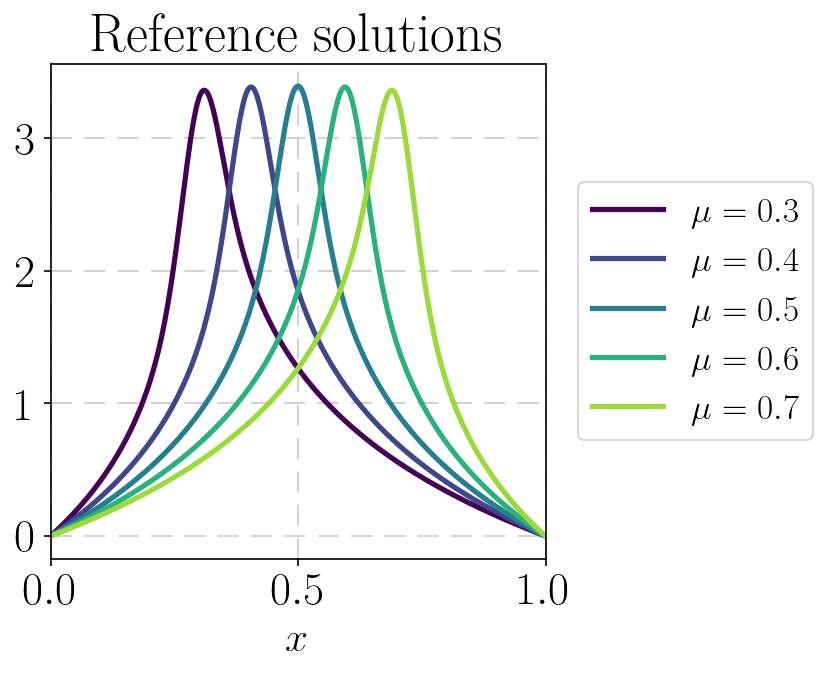
\includegraphics[height=3.5cm]{images/contrib2/operator/tp_reference_solutions.png}}%
		\only<2>{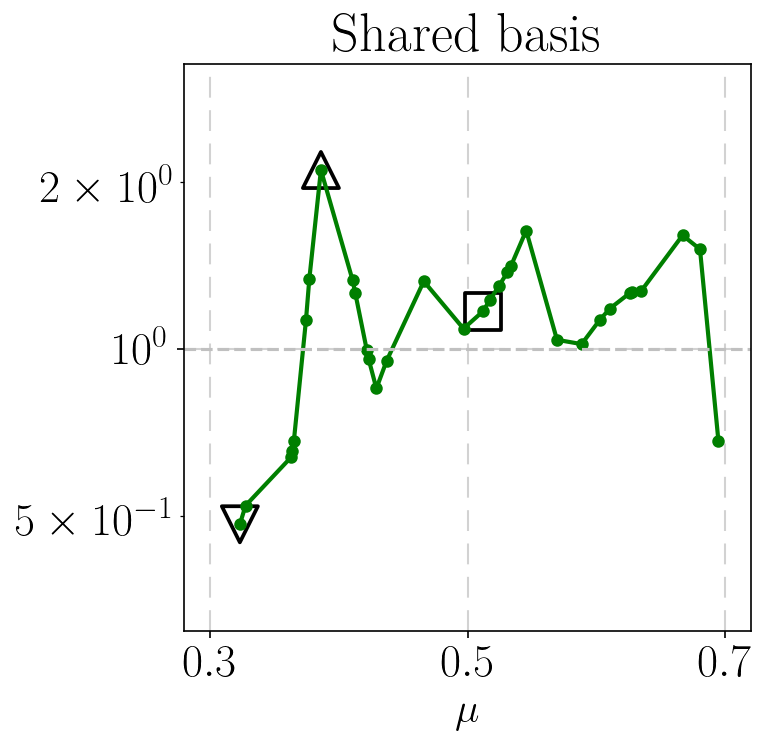
\includegraphics[height=3.2cm]{images/contrib2/operator/tp_gain_map_shared.png}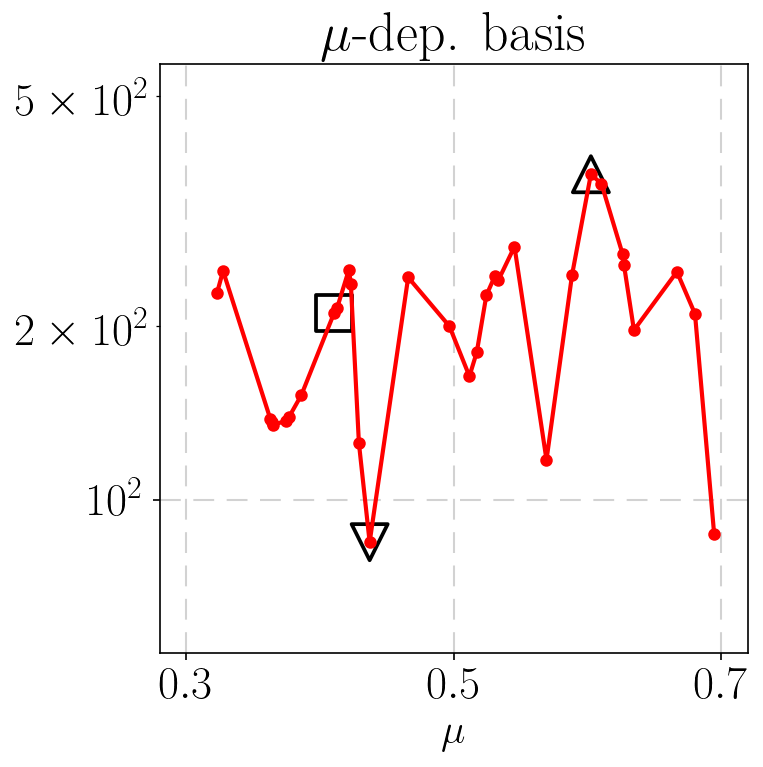
\includegraphics[height=3.2cm]{images/contrib2/operator/tp_gain_map_mu.png}\\[2pt]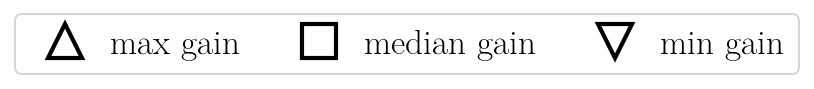
\includegraphics[height=0.5cm]{images/contrib2/operator/lt_gain_map_legend.png}}%
		\only<3->{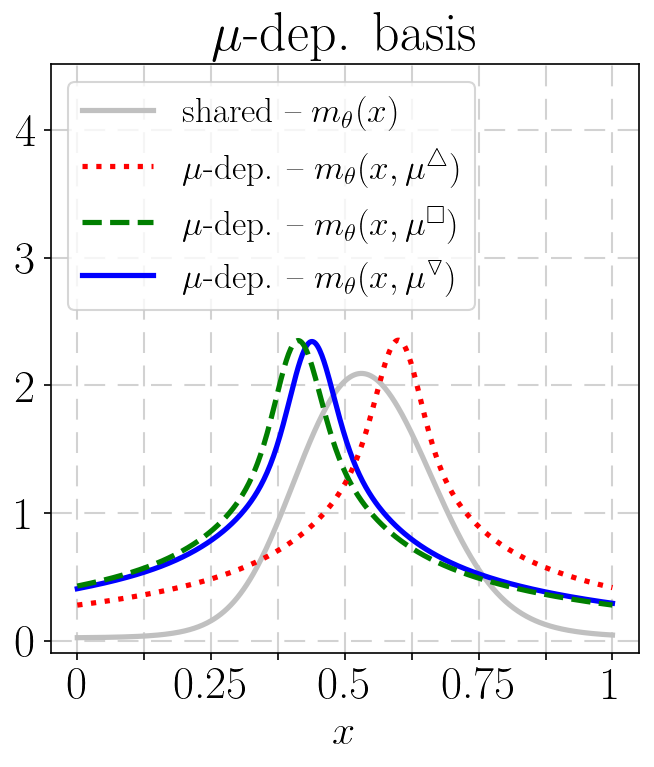
\includegraphics[height=3.7cm]{images/contrib2/operator/tp_multipliers_mu.png}}%
	}

	\vspace{2pt}
	\blk{2}{%
		\textbf{Gain (on $32$ unseen $\mu$):} \\
		shared $0.5$--$2.1$ $(N_\theta=321)$, \coloredonly<2>{$\mu$-dep.\ $85$--$366$} $(N_\theta=337)$.
	}

	\vspace{2pt}
	\blk{3}{%
		\textbf{Multipliers:} shared, \coloredonly<3>{one central bump}; $\mu$-dep., a \coloredonly<3>{peak at the layer}.
	}

	% \vspace{2pt}
	% \blk*{4}{%
	% 	\textbf{Limits:} 1D, \coloredonly<4>{$32$ training values}, best of $10$ seeds, training cost not counted.
	% }
\end{frame}
